\subsection{Four-model failure mechanisms persist on independently sourced OC20 trajectories}
\label{sec:external_results}

The external benchmark yielded 1,536 unique responses per model (6,144 total), without missing or duplicate request identifiers. Five SmolLM responses were truncated. A frozen public-evidence enumerator reconstructed all 1,536 sealed proof lists. We additionally audited the archived coordinates using independently written code: all 144 stored-frame mobile, adsorbate and fixed-atom RMSDs for 48 physical systems were reproduced to within $10^{-6}$~\AA; a separate bond-graph, periodic-unwrapping, and Kabsch implementation reproduced all 48 internal RMSDs, including the 33 multi-atom adsorbates. These independent calculations verify the archived numbers, but do not establish that the heuristic bond definitions are chemically complete. Figure~\ref{fig:external_geometry} illustrates the distinct physical meanings of the two external RMSD measures.

\begin{figure}[tbp]
  \centering
  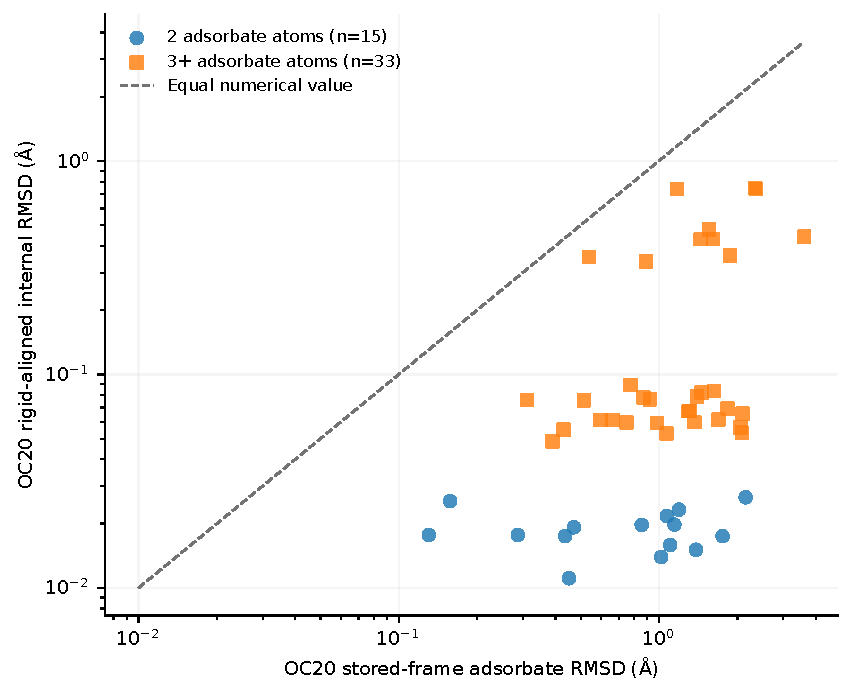
\includegraphics[width=0.75\linewidth]{figure_04.pdf}
  \caption{External OC20 physical measurement definitions for 48 independently sourced stored relaxation pairs. The stored-frame adsorbate RMSD and rigid-aligned internal RMSD need not agree because alignment removes rigid movement. Circles represent two-atom adsorbates; squares represent three or more atoms. This is the external set, not a reconstruction of the original 55 systems.}
  \label{fig:external_geometry}
\end{figure}


Table~\ref{tab:external} separates strict-format model performance from a diagnostic that removes only outer code fences. On 960 answerable questions, the fence-normalized 32B model produced 567 valid proofs (59.1\%), compared with 245 (25.5\%) for Qwen3-4B. The difference was 33.5 percentage points (95\% source-group bootstrap interval 30.4--36.7 points); this comparison is descriptive rather than a controlled scaling study. Strict-format success for Qwen3-32B was zero because every answer had a Markdown code fence. Its normalized result is therefore \emph{not} a strict-contract score. The operation-only diagnostic recovered additional proofs for every model, but still failed when a model selected the wrong endpoint or physical measurement.

\begin{table}[tbp]
\centering\small
\caption{External OC20 valid scientific proofs (960 answerable cases per model). Strict and fence-normalized model-only scores are distinct. The final column permits oracle-assisted operation replacement on an unchanged model-selected evidence identifier; it is not standalone model performance.}
\label{tab:external}
\begin{tabular}{lrrr}
\toprule
Model & Strict & Fence-normalized & After operation repair\\
\midrule
Qwen3-4B & 245 (25.5\%) & 245 (25.5\%) & 593 (61.8\%)\\
Phi-4-mini & 82 (8.5\%) & 97 (10.1\%) & 284 (29.6\%)\\
SmolLM3-3B & 1 (0.1\%) & 143 (14.9\%) & 260 (27.1\%)\\
Qwen3-32B-AWQ & 0 (0.0\%) & 567 (59.1\%) & 723 (75.3\%)\\
\bottomrule
\end{tabular}
\end{table}

\begin{figure}[tbp]
  \centering
  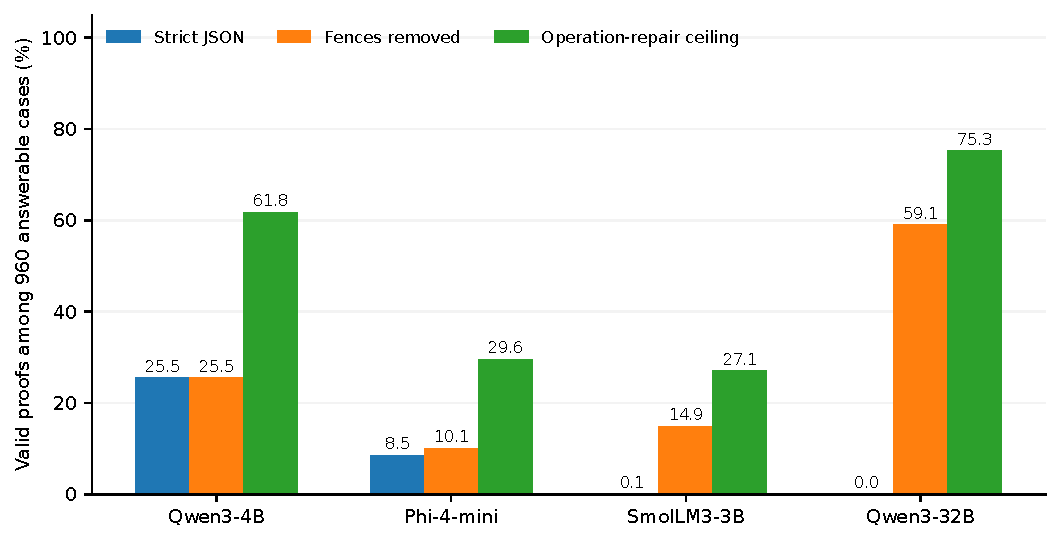
\includegraphics[width=\linewidth]{figure_05.pdf}
  \caption{Four-model proof validity on the external OC20 benchmark (960 answerable questions per model). Strict output parsing, outer-code-fence normalization, and oracle-assisted operation repair are distinct evaluations; the last two are diagnostic, not primary strict-contract results.}
  \label{fig:external_model_comparison}
\end{figure}

Among 960 answerable cases, Qwen3-32B produced 156 correct-evidence/wrong-operation selections, 131 wrong-endpoint choices, and 106 wrong or inconclusive measurement choices, in addition to 567 licensed proofs. It correctly used the evidence on 348 of 480 structured cases and 219 of 480 written-report cases; both presentations were correct for only 172 of 480 paired base cases. No model produced the required explicit scientific abstention on any of the 576 insufficient-evidence cases per model. A rejected proof was \emph{not} counted as a correct abstention. The presentation-specific error types are shown in Fig.~\ref{fig:external_error_types}.

\begin{figure}[tbp]
  \centering
  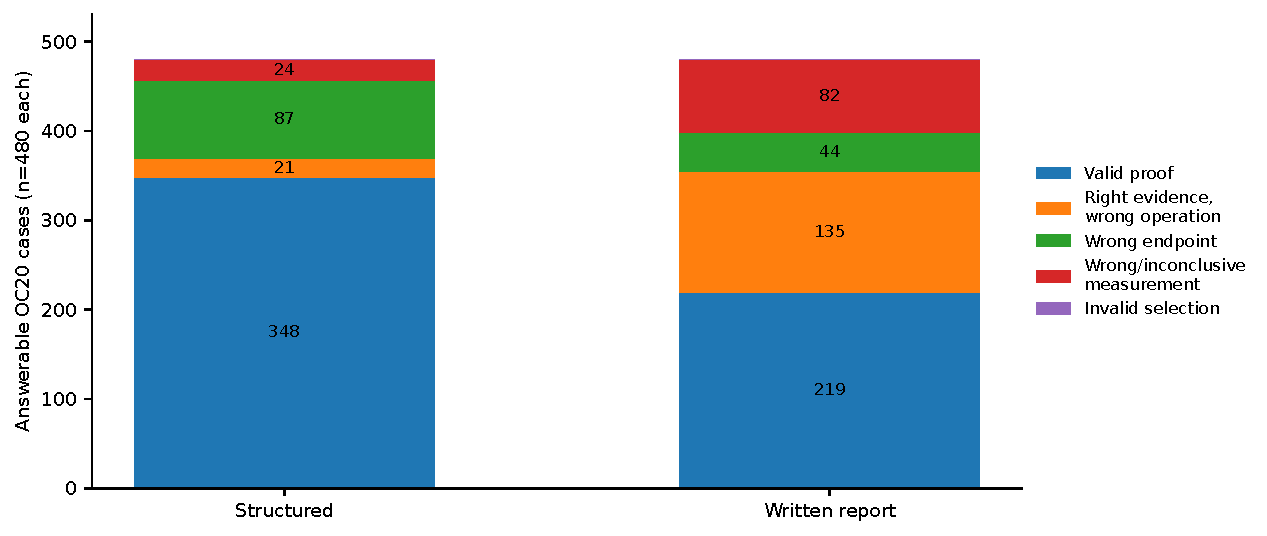
\includegraphics[width=0.88\linewidth]{figure_06.pdf}
  \caption{Qwen3-32B errors in structured and written OC20 presentations. Each presentation contains 480 answerable questions. A correct physical evidence ID with an incorrect operation is separated from a wrong endpoint comparison and a wrong physical measurement. Output code fences have been normalized for this diagnostic.}
  \label{fig:external_error_types}
\end{figure}


\subsection{High token likelihood is not a certificate of valid scientific evidence}
\label{sec:confidence_results}

The confidence replay recovered exactly the original 6,144 predictions. Decision-token scores ranked correct and incorrect answerable proofs better than chance for some models (Table~\ref{tab:confidence}). Qwen3-32B obtained AUROC 0.724 (95\% cluster-bootstrap interval 0.696--0.753), compared with 0.636 for Qwen3-4B, 0.552 for Phi, and 0.567 for SmolLM. Its most confident decile contained 90 valid and six invalid proofs among 96 eligible answers. However, among 601 Qwen3-32B answers with decision-token geometric mean above 0.99, 185 were scientifically invalid (30.8\%). This is not a formal miscalibration rate: token-generation likelihood has not been mapped to probability of scientific validity.

\begin{table}[tbp]
\centering\small
\caption{Confidence-based ranking on answerable OC20 cases. AUROC compares token confidence with licensed-proof correctness. Top-decile accuracy excludes missing decision-token scores. Confidence is not a calibrated probability of scientific truth.}
\label{tab:confidence}
\begin{tabular}{lrrr}
\toprule
Model & Score available & AUROC (95\% interval) & Top-decile valid\\
\midrule
Qwen3-4B & 960/960 & 0.636 (0.589--0.682) & 68/96\\
Phi-4-mini & 918/960 & 0.552 (0.484--0.626) & 18/92\\
SmolLM3-3B & 735/960 & 0.567 (0.507--0.620) & 22/74\\
Qwen3-32B-AWQ & 960/960 & 0.724 (0.696--0.753) & 90/96\\
\bottomrule
\end{tabular}
\end{table}

For Qwen3-32B, AUROC was 0.749 on structured cases and 0.647 on written reports, consistent with a presentation-dependent usefulness of confidence ranking. These are descriptive subgroup differences in correlated case pairs. The ROC results are restricted to answerable cases and cannot demonstrate recognition of insufficient evidence or reliable autonomous abstention. Figure~\ref{fig:confidence_revised} illustrates the ranking-versus-certification distinction.

\begin{figure}[tbp]
  \centering
  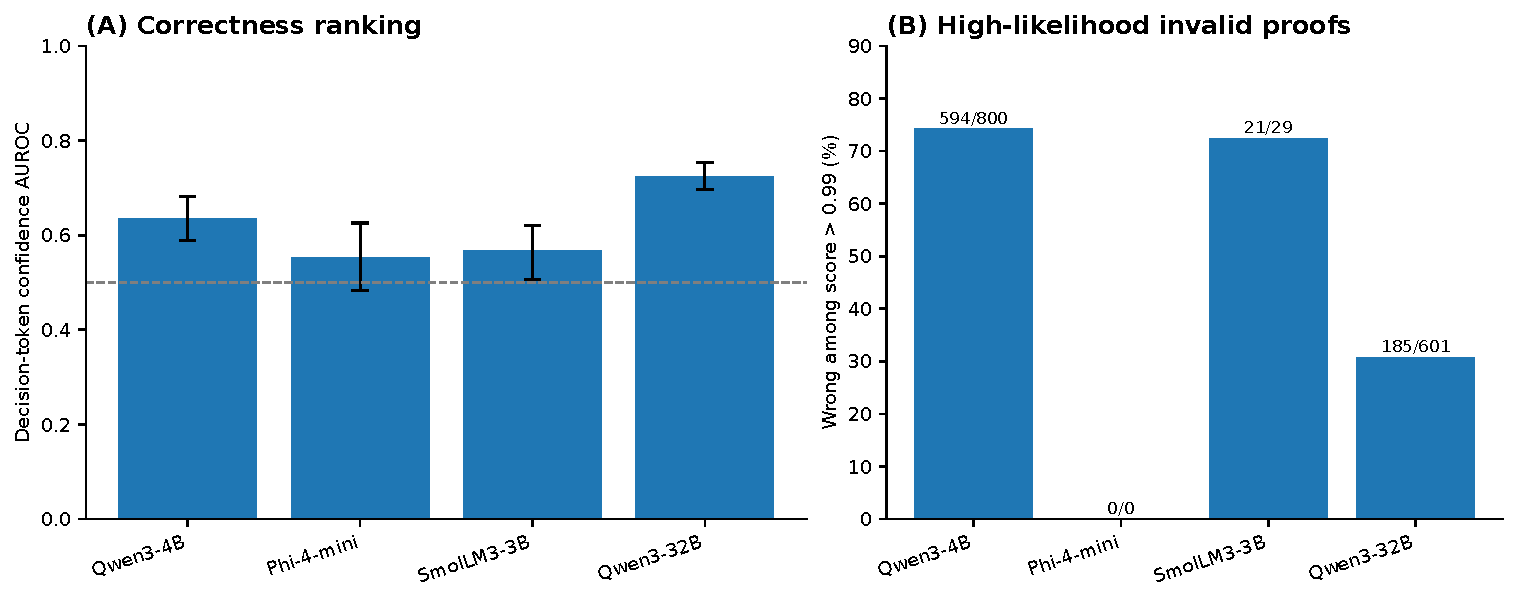
\includegraphics[width=\linewidth]{figure_07.pdf}
  \caption{Token confidence versus scientific correctness for the four models on answerable external cases. (A) Decision-token AUROC with 95\% source-group bootstrap intervals; 0.5 indicates chance-level ranking. (B) Fraction scientifically wrong among outputs with decision-token geometric mean above 0.99; Phi has no such outputs. These likelihoods are not calibrated probabilities of valid scientific proofs.}
  \label{fig:confidence_revised}
\end{figure}

